\section{Skills in the Wild}
\label{sec:insight}

\begin{figure*}[t]
  \centering
  \setlength{\abovecaptionskip}{0pt}
  \setlength{\belowcaptionskip}{-8pt}
  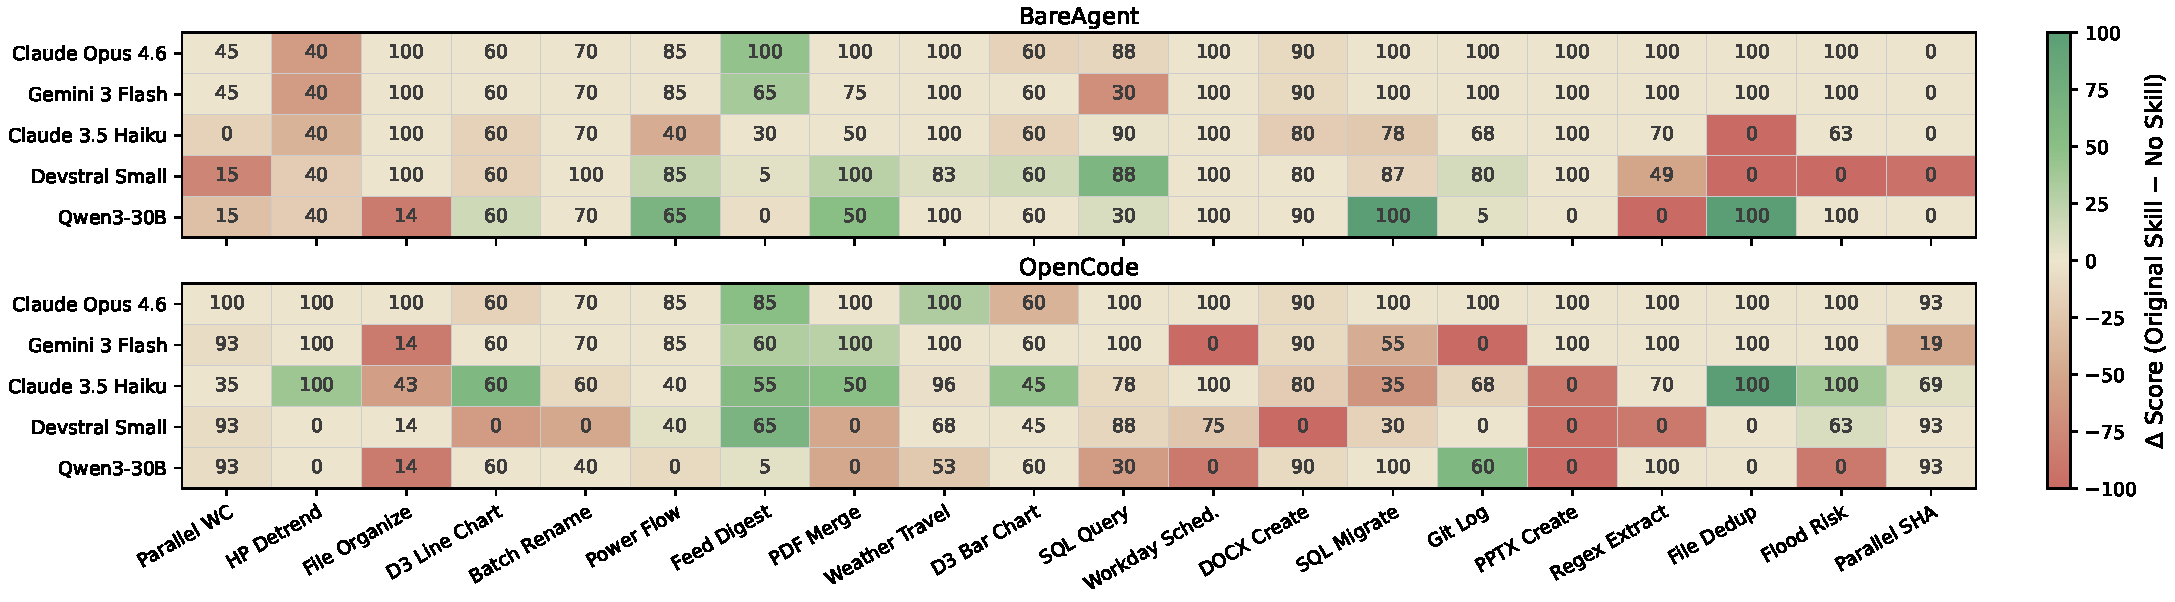
\includegraphics[width=\textwidth]{figures/m2_cross_harness_heatmap.pdf}
  \caption{Skill performance across models and harnesses.
    Columns are tasks, rows are models, and each subplot corresponds to one harness.
    Cell colors indicate score deltas relative to the no-skill baseline,
    and cell labels show absolute task scores.
    Both model identity and harness choice significantly affect outcomes.}
  \label{fig:m2_heatmap}
\end{figure*}


In this section, we first introduce skills, the agent that uses them,
and how skills are invoked in practice.
We study the skill ecosystem at scale through more than 110,000 skills
collected from two major distribution platforms:
clawhub.ai~\cite{clawhub} (28,990 skills) and skills.sh~\cite{skillssh} (89,280 skills).
Based on this ecosystem analysis, we further conduct experiments to
identify concrete problems in current skill usage.

\subsection{Skill Definition}
\label{sec:back:skills}

A \emph{skill} is a distributable, self-contained knowledge pack that
enhances an AI agent's capability on a specific class of
tasks~\cite{claude-agent-skills, agentskills-spec}.
A skill may introduce knowledge the base model does not have, or
constrain the model toward a prescribed workflow when it already
has the relevant capability but would otherwise improvise.
For example, a PDF-processing skill~\cite{anthropic-skills-repo} teaches the model how to use pdfplumber for table
extraction, and also constrains the model to use pypdf instead of the deprecated PyPDF2 when merging PDF files.

A skill is typically defined in a structured file comprising three
layers:
(1)~\emph{metadata}---a name, description, and trigger conditions
that allow the agent runtime to discover and select the skill automatically;
(2)~\emph{instructions}---the main body of a skill that encodes
multi-step workflows, tool references, and other task-specific guidance
in natural language; and
(3)~\emph{bundled resources}---scripts, references, and
templates stored in companion files.

This structure distinguishes skills from ad-hoc prompt snippets.
The metadata makes a skill a discoverable, selectable unit, enabling the
agent runtime to match tasks to applicable skills automatically rather than
requiring manual prompt assembly~\cite{claude-code-skills}.
Compared with fine-tuning, skills require no weight modification
and can be operated entirely at the prompt level~\cite{ouyang2022training, liu2021pretrain}, making them lightweight to
distribute and easy to compose.
Multiple agent platforms have converged on this
abstraction~\cite{claude-code-skills, cursor-skills, openai-codex-cli, agentskills-spec, antigravity-skills, coze-skills}, and existing
tools support basic skill authoring, management, and optimization.

\subsection{LLM Agent and Agent Harness}
\label{sec:back:harness}

An LLM agent works in a ReAct loop~\cite{yao2023react}. It receives a task, reasons
about what to do, issues a tool call (reading a file, running
a command, making an API request)~\cite{schick2023toolformer, openai2023functioncalling}, observes the result, and
reasons again. This loop repeats until the task is done.

The agent does not interact with the outside world directly.
It runs inside an \emph{agent harness}, a runtime framework
that sits between the model and the operating environment~\cite{wu2023autogen, langgraph}.
The harness manages the LLM API connection, registers the
tools the agent can call, dispatches those calls, and controls
how much conversation history fits in the context window.
Claude Code~\cite{claudecode}, OpenCode~\cite{opencode}, and OpenClaw~\cite{openclaw} are examples of widely used
harnesses.

Harnesses differ in ways that matter for skills~\cite{google-a2a}.
Some provide a rich set of file-system and web search tools,
while others expose only basic read, write, and shell execution operations.
Some can spawn independent sub-agents that work concurrently,
while others only support sequential execution.
These differences directly affect whether a skill's instructions can be carried out.

\subsection{Characterizing Skills}
\label{sec:insight:analysis}

\heading{Ecosystem Scale and Distribution.}
The skill ecosystem is large but uneven.
Figure~\ref{fig:skill_distribution} shows the download counts
across both platforms. On skills.sh, 89\% of the 89,280 skills
have fewer than 86 downloads, while a handful of head skills
reach $10^4$--$10^6$. clawhub.ai follows a similar long-tailed
pattern, peaking around $10^2$--$10^3$ downloads. In total,
over 118,000 skills exist across the two platforms, but the
vast majority see little use.
\begin{figure}[t]
  \centering
  \setlength{\abovecaptionskip}{0pt}
  \setlength{\belowcaptionskip}{-10pt}
  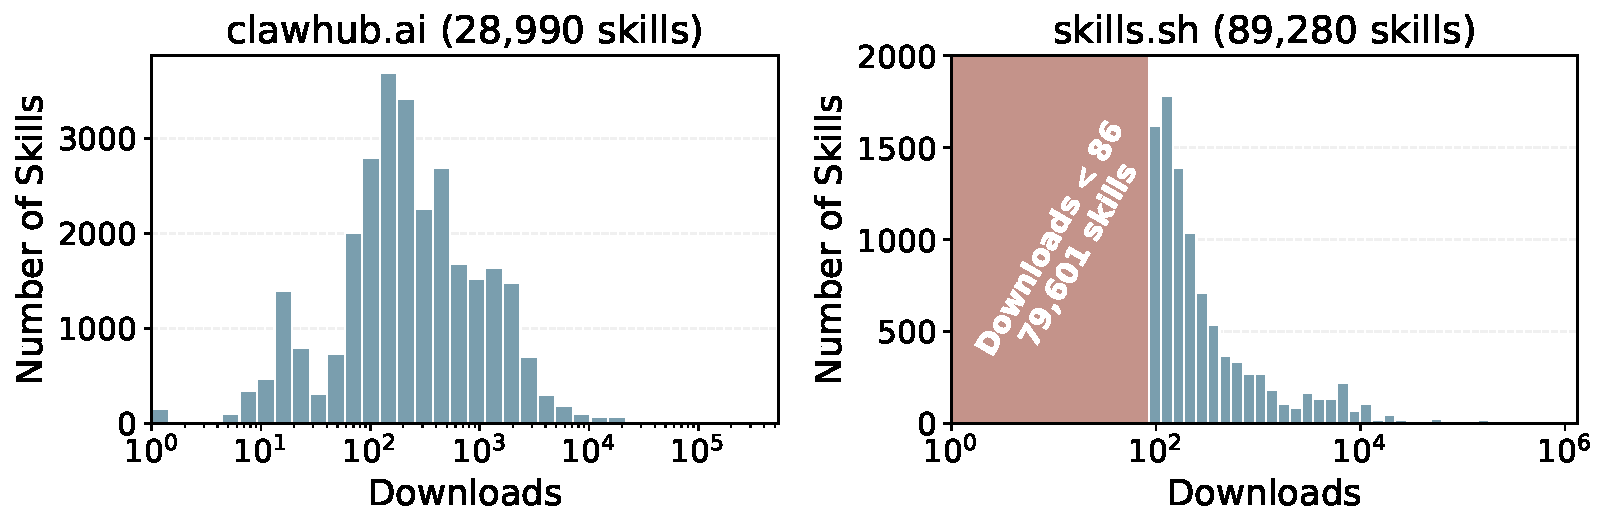
\includegraphics[width=\columnwidth]{figures/skill_download_distribution.pdf}
  \caption{Skill download distribution on clawhub.ai and
    skills.sh. Both platforms show a long-tailed distribution.}
  \label{fig:skill_distribution}
\end{figure}

\heading{Skill Taxonomy.}
Skills differ substantially in what they provide the agent with.
We use LLM-assisted analysis to classify 15,063 skills that have
more than 100 downloads into three categories, based on which
aspect the skill most emphasizes: tool reference (52\%),
procedural guidance (28\%), and content generation (20\%).

\emph{Tool-reference skills} teach the model how to
operate specific tools, APIs, or CLIs. They are essentially
usage documentation loaded into the agent's context.
A representative example is a skill that documents
how to use python to merge, split, and manipulate PDF files.

\emph{Procedural skills} prescribe step-by-step
workflows and reasoning strategies for carrying out a task.
A representative example is a debugging skill that enforces
a four-phase process: reproduce the failure, trace the root
cause, apply a targeted fix, and verify the fix with tests.

\emph{Generative skills} ask the model to produce
content, code, documents, or prose. The core quality depends
on the model's own capability. An example is a
frontend-design skill~\cite{anthropic-skills-repo} that generates production-grade web
components with specific design guidelines and styling
conventions.

Tool-reference and procedural skills together account for
80\% of the ecosystem. These skills encode analyzable
structure, including script fragments and step-by-step workflows.
The correctness of executing these skills depends
on whether the agent executes the prescribed steps, not on
its generative ability.

\heading{Workflow Structure.}
Beyond task type, skills also exhibit repeated internal
structure. Across the 15,063 classified skills, 76\%
contain explicit procedural structure: numbered steps,
conditional branches, and data dependencies between steps.

\heading{Code Fragments.}
75\% of skills embed code-like fragments: shell
commands, API call patterns, or script snippets whose overall
shape recurs across invocations while only the input-specific
parameters change.
For example, a weather skill~\cite{openclaw} may provide a family of curl command
templates for current conditions, forecasts, and format options, where
the command structure stays fixed while parameters such as the city,
output format, and forecast day vary.


\subsection{Problems with Current Skill Usage}
\label{sec:insight:problems}

Skills are loaded into the agent's context as raw text, with no adaptation.
But skills carry implicit assumptions about the model, agent harness, and user environment.
When those assumptions are wrong, three failure modes emerge.

\heading{P1: Model Mismatch.}
A skill implicitly assumes that the model is capable enough
to follow its instructions. In practice, models differ
dramatically~\cite{lu2024agentbench}. 
Figure~\ref{fig:m2_heatmap} shows scores for
a subset of tasks across three models and three harnesses.\footnote{BareAgent is a minimal agent harness that we built. It implements only basic agent runtime logic and exposes only read, write, and exec tools.}
Performance varies substantially across models on the same skill.
Moreover, enabling skills degrades performance on 15\% of tasks; leaves scores unchanged on 17\% of tasks (excluding tasks with a 100\% completion rate); and yields no improvement for at least one model on 87\% of tasks.
\begin{examplebox}
\textbf{Case Study:} the pptx-creation skill~\cite{anthropic-skills-repo}
recommends PptxGenJS (a javascript library) for slide generation.
Claude-opus-4.6 and gemini-3-flash both score 100 with this skill,
but devstral-small misreads PptxGenJS as a CLI when using OpenCode
and repeatedly executes wrong commands.
Without the skill, devstral-small instead uses python-pptx and scores 95.
The skill assumes a model can distinguish a library API from a CLI,
which holds for frontier models but not weaker ones.
\end{examplebox}


\heading{P2: Harness Mismatch.}
The same model produces different results on the same task depending on the agent harness it runs in~\cite{yang2024sweagent}.
Figure~\ref{fig:m2_heatmap} also shows this dimension:
across the heatmap, harness-induced variance is comparable to model-induced variance.
Skills are written without knowledge of what tools and plugins the harness provides.

\begin{examplebox}
\textbf{Case Study:} Gemini 3 Flash scores 100 on the workday-scheduling task
with the original skill on BareAgent, but 0 on OpenCode with the same skill.
The failure is triggered by a malformed JSON key that makes the output
unparseable. BareAgent adds only a minimal system prompt, whereas
OpenCode prepends extensive tool documentation, and the longer combined
context induces the formatting error.
\end{examplebox}

\heading{P3: Environment Mismatch.}
Skills have dependencies on the execution environment, but
the user's machine may lack the required packages, tools, or
configurations.
Some skills list prerequisites, but those instructions are often general and target
a generic machine rather than the user's actual setup. The
real requirement depends on the current OS, hardware, installed
versions, and package-manager state.
Other skills omit the dependency entirely.
Figure~\ref{fig:p3_env_motivation} shows the effect on two
representative tasks. When the required library is absent,
both Qwen models drop to 33--67\% success rate while
generating 2--4$\times$ more output tokens on failed
workarounds. Even Claude~Opus~4.6, which still succeeds on
every run, generates 56--69\% more output tokens because it
must diagnose the mismatch and install the missing package
at runtime. Leaving diagnosis to the model therefore turns
every missing dependency into a repeated tax on both
correctness and efficiency.

\begin{figure}[t]
  \centering
  \setlength{\abovecaptionskip}{3pt}
  \setlength{\belowcaptionskip}{0pt}
  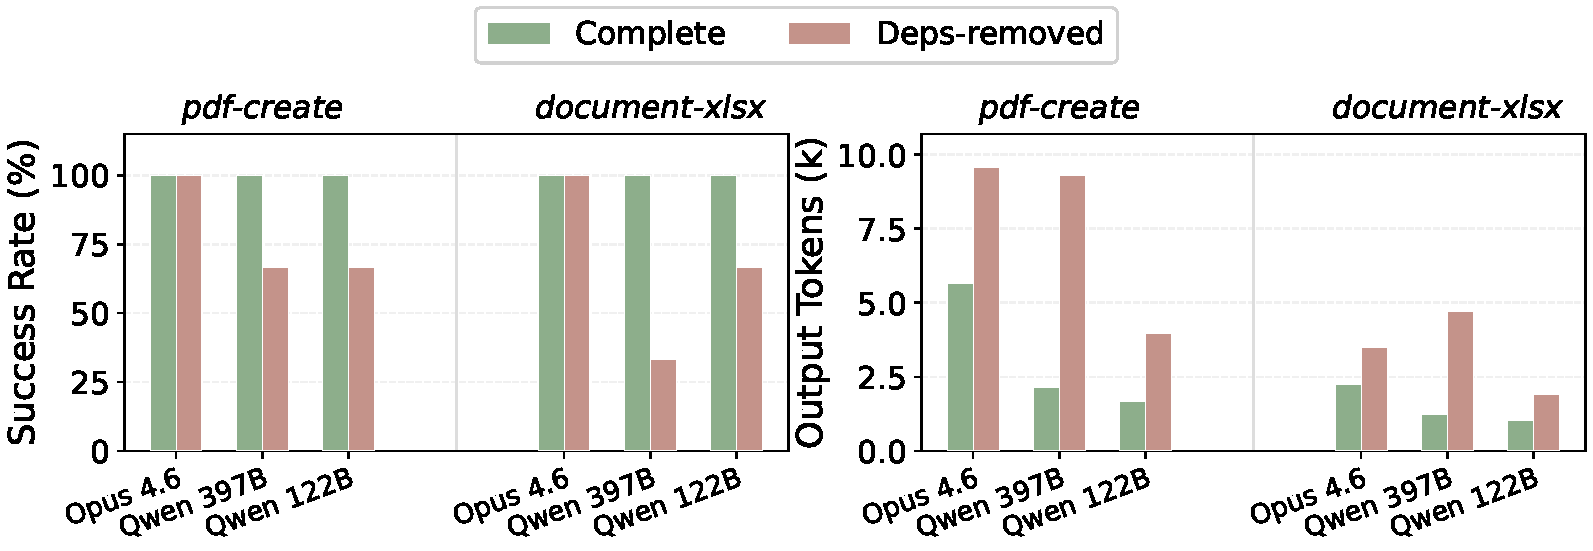
\includegraphics[width=\columnwidth]{figures/p3_env_binding_motivation.pdf}
  \caption{Removing a required dependency hurts both correctness and efficiency.}
  \label{fig:p3_env_motivation}
\end{figure}

\subsection{Challenges}
\label{sec:insight:challenges}

Skills are distributed as plain Markdown so that any agent can load them with no special tooling.
The mismatches above undermine this portability promise.
Restoring portability requires adapting each skill to its
target, which is challenging for two reasons.

\heading{C1: Targets Differ Along Many Axes.}
Each of the three dimensions above, model, harness, and
environment, varies independently. A skill that needs
adaptation along one dimension may need a different adaptation
when two dimensions change together. The right fix for a weak
model on a rich harness differs from the right fix for the
same model on a minimal one. This interaction makes the
adaptation space combinatorial: it cannot be covered by a
fixed set of rewrite rules.

\heading{C2: Skills Are Unstructured Natural Language.}
Source code requires compilation before it can run on a target system,
and has a grammar, types, and a well-defined AST that tools can analyze~\cite{aho2006compilers}.
In comparison, skills are written in natural language.
Although skills are mostly created following common conventions,
different skills vary widely in structure, terminology, and level of detail.
Before any adaptation can happen, the skill's implicit requirements and workflow structure
must be recovered from prose.